
\documentclass[12pt]{article}
\usepackage{amsmath}
\DeclareMathOperator*{\argmin}{arg\,min} % thin space, limits underneath in displays
\DeclareMathOperator*{\argmax}{arg\,max} % thin space, limits underneath in displays
\newtheorem{thm}{Theorem}
\usepackage{amssymb}
\usepackage{amsfonts}
\usepackage{mathrsfs}
\usepackage{bm}
\usepackage{indentfirst}
\setlength{\parindent}{0em}
\usepackage[margin=1in]{geometry}
\usepackage{graphicx}
\usepackage{setspace}
\doublespacing
\usepackage[flushleft]{threeparttable}
\usepackage{booktabs,caption}
\usepackage{float}
\usepackage{graphicx}
\usepackage[sort,comma]{natbib}
\usepackage[hidelinks]{hyperref}

\usepackage{import}
\usepackage{xifthen}
\usepackage{pdfpages}
\usepackage{transparent}

\newcommand{\incfig}[1]{%
\def\svgwidth{\columnwidth}
\import{./figures/}{#1.pdf_tex}
}




\title{Endogenous Growth model}
\author{}
\date{}


\begin{document}
\maketitle

Endogenous growth model differs from Ramsey's and Diamond's model in explicitly 
interpreting the effectiveness of labor as knowledge and in modeling the determinants
of its evolution over time. Romer's model is one specific endogenous growth model.



\section{Assumptions}
1. Two sectors, goods-producing sector (output), and R\&D sector (knowledge and idea).

2. 
\begin{align*}
		\alpha_{L}&: \text{ fraction of labor is used in the R\&D }\\
		1 - \alpha_{L}&: \text{ fraction of labor is used in goods production }\\
		\alpha_{K}&: \text{ fraction of capital is used in the R\&D }\\
		1 -  \alpha_{K}&: \text{ fraction of capital is used in the goods production }
\end{align*}
$ \alpha_{L} $ and $ \alpha_{K} $ are exogenous and constant, and are between 0 and 1.


3. Production function:
\begin{equation*}
Y(t) = \left[ (1 - \alpha_{K}) K(t) \right] ^{\alpha}
\left[ A(t)(1 - \alpha_{L})L(t) \right] ^{1 - \alpha}
\end{equation*}


4. Production of new idea:
\begin{equation*}
		\dot{A}(t) = B[\alpha_{K}K(t)]^{\beta}[\alpha_{L}L(t)]^{\gamma}A(t)^{\theta},
		\quad B > 0, \beta, \gamma \ge 0
\end{equation*}
where $ B $ is a shift parameter.
{\textbf {Note}}, it is {\textbf {not}} necessary that $ \beta + \gamma + \theta =1 $.


5. No depreciation.
\begin{equation*}
\dot{K}(t) = sY(t), \quad 0 < s < 1
\end{equation*}

6. Population grows exogenously at $ n $.
\begin{equation*}
\dot{L}(t) = n L(t), \quad n \ge 0
\end{equation*}




\section{Model without capital}
\begin{align*}
\text{ Goods production }&: Y(t) = A(t)(1 - \alpha_{L})L(t)\\
\text{ Idea production }&: \dot{A}(t) = B[\alpha_{L}L(t)]^{\gamma}A(t)^{\theta}
\end{align*}
The goods production says output per worker, $ \frac{Y}{L} $ is proportional to $ A $.
Thus the growth rate of $ \frac{Y}{L} $ is the growth rate of $ A $, which is $ g_{A} $.

So, we want to know 1) what is $ g_{A} $ and 2) how does change over time.

{\textbf {What is $ g_{A} $}}:
\begin{align}
g_{A}(t) &= \frac{\dot{A}(t)}{A(t)}\\
\label{eqn:ga}
&= B(\alpha_{L}L(t))^{\gamma} A(t)^{\theta - 1}
\end{align}

{\textbf {How does $ g_{A} $ change}}:\\
Take log then differentiate it wrt time $ t $.
\begin{align*}
\ln g_{A}(t)&= \ln B + \gamma \ln \alpha_{L} + \gamma \ln L(t) + (\theta - 1)\ln A(t)\\
\frac{\dot{g}_{A}(t)}{g_{A}(t)} = \frac{\partial \ln g_{A}(t) }{\partial t }
&= \gamma \frac{\dot{L}(t)}{L(t)} + (\theta - 1)\frac{\dot{A}(t)}{A(t)}\\
&= \gamma n + (\theta - 1)g_{A}(t)
\end{align*}
Change of the growth rate of knowledge:
\begin{equation}
		\label{eqn:change of ga}
\dot{g}_{A}(t) &= \gamma n g_{A}(t) + (\theta - 1)[g_{A}(t)]^{2}
\end{equation}
From equation \eqref{eqn:ga}, $ g_{A}(t) $ is determined by $ A $, $ L $ and other 
parameters. And $ g_{A}(t) $ determines the change, $ \dot{g}_{A}(t) $.



\subsection{Case 1: $ \theta < 1 $}
It says the more knowledge stock, the harder for us to discover new knowledge.

Solve for two solutions and plot equation \eqref{eqn:change of ga}
\begin{align*}
		\dot{g}_{A}(t) = 0 &= \gamma n g_{A}(t) + (\theta - 1)[g_{A}(t)]^{2}\\
g_{A}^{*} = 0,& \quad g_{A}^{*} = \frac{\gamma n}{1 - \theta}
\end{align*}

\begin{figure}[H]
\center{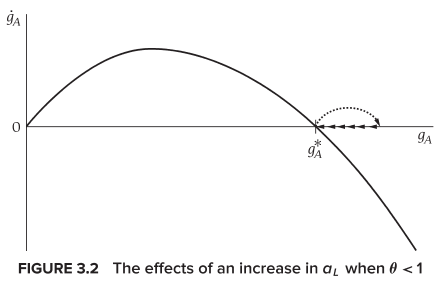
\includegraphics[scale =.5 ]  {figures/endogenous_growth_theta_less_1.png}}
\end{figure}



It says if initial $ g_{A}(0) $ is less than $ g_{A}^{*} $, $ \dot{g}_{A} > 0$,
growth rate will increase to the SS level, $ g_{A}^{*} $.

If initial $ g_{A}(0) $ is greater than $ g_{A}^{*} $, $ \dot{g}_{A} < 0$,
growth rate will reduce to the SS level, $ g_{A}^{*} $.

Because the output per worker is determined by the growth rate of A, the change in
$ g_{A}(t) $ will affect the growth rate of output per worker, $ \frac{Y}{L} $.\\


{\textbf {Shocks (An increase in $ \alpha_{L} $):}}

Consider we start at SS level $ g_{A}^{*} $.

From equation \eqref{eqn:ga}
\begin{equation*}
		g_{A}(t) = B[\alpha_{L}L(t)]^{\gamma}A(t)^{\theta - 1}
\end{equation*}
If there is an increase in $ \alpha_{L} $, $ g_{A}(t) $ will increase immediately (
the growth rate of A). Then, according to Figure 3.2, the growth rate will gradually
decrease to the SS level, $ g_{A}^{*} $. So, the change in $ \ln A $ would be

\begin{figure}[H]
\center{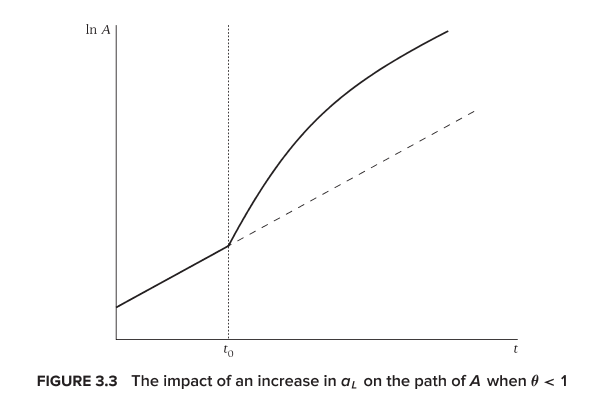
\includegraphics[scale =.5 ]  {figures/change_in_alpha_L.png}}
\end{figure}

$ \alpha_{L} $ does not affect the growth rate at SS level.


\subsection{Case 2: $ \theta > 1 $}
\begin{align*}
		\dot{g}_{A}(t) &= \gamma n g_{A}(t) + (\theta - 1)[g_{A}(t)]^{2}\\
		g_{A}^{*} = 0,& \quad g_{A}^{*} =  \frac{\gamma n}{1 - \theta} < 0 
\end{align*}
The negative root is meaningless. So $ g_{A}^{*} = 0 $.

\begin{figure}[H]
\center{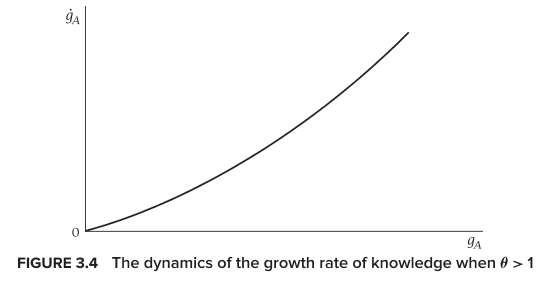
\includegraphics[scale =.5 ]  {figures/endogenous_growth_theta_greater_1.png}}
\end{figure}

\subsection{Case 3: $ \theta = 1 $}
\begin{align*}
		g_{A}(t)&= B[\alpha_{L}L(t)]^{\gamma}\\
		\dot{g}_{A}(t)&= \gamma n g_{A}(t)
\end{align*}




\section{The General Model}
Now we have two endogenous state variables, $ A $ and $ K $.


\begin{align*}
Y(t) &= \left[ (1 - \alpha_{K}) K(t) \right] ^{\alpha}
\left[ A(t)(1 - \alpha_{L})L(t) \right] ^{1 - \alpha}\\
\dot{A}(t) &= B[\alpha_{K}K(t)]^{\beta}[\alpha_{L}L(t)]^{\gamma}A(t)^{\theta}\\
\dot{K}(t) &= sY(t)
\end{align*}

Plug $ Y(t) $ into capital accumulation function,
\begin{equation*}
\dot{K}(t) = s(1 - \alpha_{K})^{\alpha}(1 - \alpha_{L})^{1 - \alpha}
K(t)^{\alpha}A(t)^{1 - \alpha}L(t)^{1 - \alpha}
\end{equation*}

{\textbf {What is $ g_{K}(t) $:}\

Derive the growth rate of capital, $ g_{K}(t) $,
\begin{align*}
g_{K}(t)&= \frac{\dot{K}(t)}{K(t)}\\
&= c_{K}
\left[ \frac{A(t)L(t)}{K(t)}\right] ^{1 - \alpha}
\end{align*}
where $ c_{K} = s(1 - \alpha_{K})^{\alpha}(1 - \alpha_{L})^{1 - \alpha} $.


{\textbf {How does $ g_{K}(t) $ change:}}

Take log and differentiate wrt $ t $,
\begin{align*}
		\ln g_{K}(t) &= \ln c_{K} + (1 - \alpha)[\ln A(t) + \ln L(t) - \ln K(t)]\\
\frac{\dot{g}_{K}(t)}{g_{K}(t)} = \frac{\partial \ln g_{K}(t) }{\partial t }
&= (1 - \alpha)(g_{A}(t) + n - g_{K}(t))
\end{align*}

We know $ g_{K} > 0 $ from the definition of $ \dot{K}(t) $.
So,

\begin{itemize}
\item growth rate of $ g_{K} $ is positive if $ g_{A} + n - g_{K} > 0 $.
\item growth rate of $ g_{K} $ is negative if $ g_{A} + n - g_{K} < 0 $.
\item growth rate of $ g_{K} $ is 0 if $ g_{A} + n - g_{K} = 0 $.
\end{itemize}


Condition for $ \dot{g}_{K} = 0 $:

\begin{equation*}
g_{K} = g_{A} + n
\end{equation*}

\begin{figure}[H]
\center{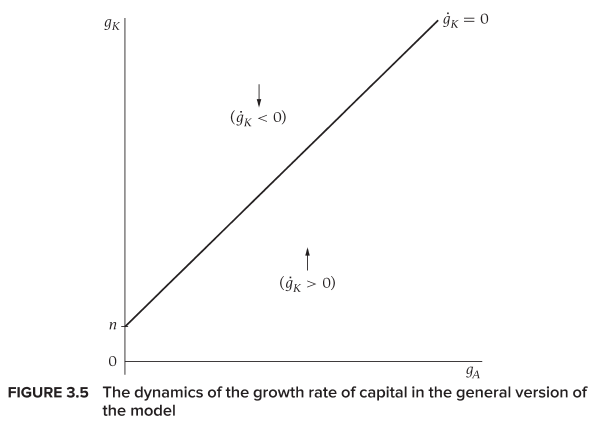
\includegraphics[scale =.5 ]  {figures/gk_gA.png}}
\end{figure}


{\textbf {Now, solve for the growth rate of $ g_{A} $:}}

Recall
\begin{align*}
\dot{A}(t) &= B[\alpha_{K}K(t)]^{\beta}[\alpha_{L}L(t)]^{\gamma}A(t)^{\theta}\\
g_{A}= \frac{\dot{A}(t)}{A(t)} &= B[\alpha_{K}K(t)]^{\beta}[\alpha_{L}L(t)]^{\gamma}
A(t)^{\theta - 1}\\
&= c_{A}K(t)^{\beta}L(t)^{\gamma}A(t)^{\theta - 1}
\end{align*}
where $ c_{A} = B \alpha_{K}^{\beta}\alpha_{L}^{\gamma} $.
Take log and differentiate it wrt $ t $, 
\begin{equation*}
\frac{\dot{g}_{A}(t)}{g_{A}(t)} = \beta g_{K}(t) + \gamma n  + (\theta - 1)g_{A}(t)
\end{equation*}

{\textbf {Suppose $ \theta < 1 $}},
at SS, 
\begin{align*}
\frac{\dot{g}_{A}(t)}{g_{A}(t)} &= \beta g_{K}(t) + \gamma n  + (\theta - 1)g_{A}(t) = 0
\\
g_{K}(t) &= \frac{(1 - \theta)g_{A}(t) - \gamma n}{\beta}
\end{align*}

\begin{figure}[H]
\center{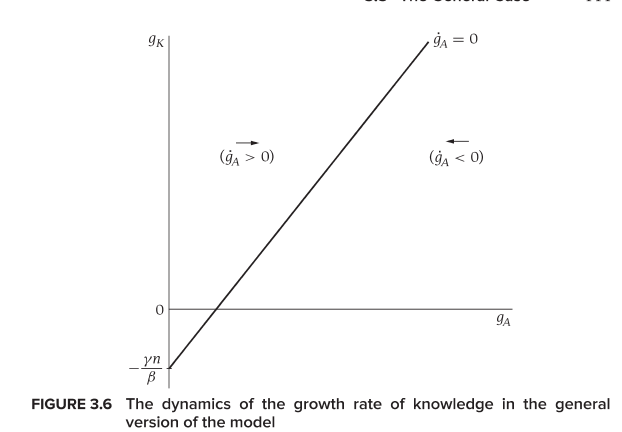
\includegraphics[scale =.7 ]  {figures/general_gk_ga.png}}
\end{figure}

Because the production function for goods is CRTS, the return to scale depends on 
how $ A $ will change, $ \dot{A}(t) $,
\begin{equation*}
\dot{A}(t) = B[\alpha_{K}K(t)]^{\beta}[\alpha_{L}L(t)]^{\gamma}A(t)^{\theta}
\end{equation*}


\subsection{$ \beta + \theta < 1 $}
If $ \beta + \theta < 1 $, then $ \beta < 1 - \theta $, and 
\begin{equation*}
\frac{1 - \theta}{\beta} > 1
\end{equation*}


\begin{equation*}
g_{K}(t) = \frac{(1 - \theta)g_{A}(t) - \gamma n}{\beta}
\end{equation*}
It says the above $ \dot{g}_{A}=0 $ condition is steeper.

Two conditions:
\begin{align*}
\text{ $ \dot{g}_{K} =  0 $ }&:
\frac{\dot{g}_{K}(t)}{g_{K}(t)} = (1 - \alpha)(g_{A}(t) + n - g_{K}(t)) =0\\
\text{ $ \dot{g}_{A} = 0 $ }&:
\frac{\dot{g}_{A}(t)}{g_{A}(t)} = \beta g_{K}(t) + \gamma n  +  (\theta - 1) g_{A}(t)
\end{align*}
\begin{align}
		\label{eqn:gk = 0}
\text{ $ \dot{g}_{K} =  0 $ }&:
g_{K}^{*} = g_{A}^{*} + n\\
\label{eqn:ga = 0}
\text{ $ \dot{g}_{A} = 0 $ }&:
g_{K}^{*} = \frac{1 - \theta}{\beta}g_{A}^{*} - \frac{\gamma n}{\beta}
\end{align}


\begin{figure}[H]
\center{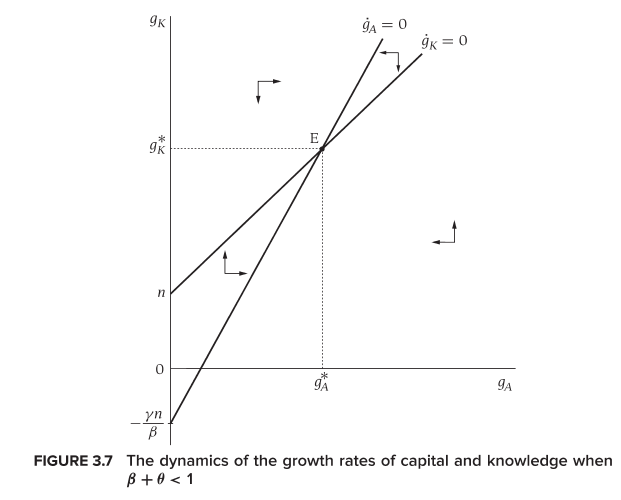
\includegraphics[scale =.5 ]  {figures/combine_ga_gk.png}}
\end{figure}

Now plug in equation \eqref{eqn:gk = 0} to equation \eqref{eqn:ga = 0} and solve for
$ g_{A}^{*} $
\begin{equation*}
g_{A}^{*} = \frac{(\beta + \gamma)n}{1 - (\theta + \beta)}
\end{equation*}

It says output per worker is growing at $ g_{A}^{*} $, output is growing at rate
$ g_{K}^{*} $

To prove this, 
\begin{align*}
Y(t) &= \left[ (1 - \alpha_{K}) K(t) \right] ^{\alpha}
\left[ A(t)(1 - \alpha_{L})L(t) \right] ^{1 - \alpha}\\
\frac{Y}{L} &= \left[ (1 - \alpha_{K})\frac{K}{L} \right]^{\alpha} 
A^{1 - \alpha}(1 - \alpha_{L})^{1 - \alpha}\\
g_{\frac{Y}{L}}&= \alpha(g_{K} - n) + (1 - \alpha)g_{A}
\end{align*}
Given $ g_{K}^{*} = g_{A}^{*} + n $, $ g_{K}^{*} - n = g_{A}^{*} $,
\begin{equation*}
g_{\frac{Y}{L}}^{*}= \alpha g_{A}^{*} + g_{A}^{*} - \alpha g_{A}^{*}= g_{A}^{*}
\end{equation*}




\section{The Romer's Model}
If knowledge is sold at MC, the creators of knowledge earn negative profit. Therefore,
Romer (1990) assumes that 

1)the developer of an idea has monopoly rights to use the idea, charge a price above MC.

2)inputs into production that embody different ideas are imperfect substitutes.

For simplicity, we assume $ \theta = 1, n = 0 $.

Model of this type exhibit no {\textbf {transition dynamics.}} In response to a shock,
the economy jumps immediately to its new stable arm.


\subsection{Assumptions}
\begin{enumerate}
\item 
$ \theta = 1, n = 0 $
\item 
Eliminate all types of physical and human capital.
\item 
There is an infinity of potential specialized inputs into production. More ideas are 
used, more output is produced.
\item 
There is a range of ideas that are currently {\textbf {available}} that extends from
0 to A. $ A > 0, \quad A = A(t) $.
\item When an idea is available, the input into production embodying the idea can be
		produced using a technology that transforms labor one-to-one into the input.
\item 		
We use $ L(i) $ to denote both the Q of labor devoted to producing input $ i $ and
the Q of input $ i $ that goes into final-goods production.
\item How inputs combine to produce final output:
		\begin{equation*}
		Y = \left[ \int_{i = 0}^{A}L(i)^{\phi } d i \right] ^{\frac{1}{\phi}}, \quad
		\phi \in (0,1)
		\end{equation*}
Remember, we have infinite number of input $ i $.
\item 
		The monopolist (patent holder) charges a constant price for each unit of the input,
		rule out price discrimination.
\item 
Output is produced by competitive firms that take the prices of inputs as given.
They sell final goods (output) at MC.
\end{enumerate}


\subsection{Cost minimization problem}
Let $ p(i) $ denote the price charged by the patent holder on idea $ i $ for each
unit of the input embodying that idea. We can write down the Lagrangian for the problem
of producing one unit of output at minimum cost is
\begin{equation*}
\mathscr{L} = \int_{i = 0}^{A} p(i)L(i)d i  +  \lambda
\left\{ 
		1 - \left[ \int_{i = 0}^{A}L(i)^{\phi}d i  \right]^{\frac{1}{\phi}} 
\right\} 
\end{equation*}

{\textbf {FOC wrt $ L(i) $:}}
\begin{equation*}
p(i) = \lambda L(i)^{\phi - 1}
\end{equation*}
we use the fact that $ \int_{i = 0}^{A}L(i)^{\phi}d i  $ must equal 1.

Rewrite the FOC,
\begin{equation*}
L(i) = \left[ \frac{\lambda}{p(i)} \right] ^{\frac{1}{1 - \phi}}
\end{equation*}
It says patent holder faces a downward-sloping demand curve.
\begin{equation*}
\varepsilon_{L} = \frac{d \ln L}{d \ln p} =  - \frac{1}{1 - \phi}
\end{equation*}
As $ \phi \rightarrow 1 $ , more elastic.



\subsection{Another Four Assumptions:}
\begin{enumerate}
\item Population is fixed, $  \overlinL{L} > 0 $. Works can produce either 1)
		intermediate goods or 2) R\&D.

		Let $ L_{A}(t) $ denote people for R\&D at time $ t $.
		\begin{equation*}
		 \overline{L} = L_{A}(t) + L_{Y}(t)
		\end{equation*}
		where 
		\begin{equation*}
		L_{Y}(t) = \int_{i = 0}^{A(t)} L(i,t)d i
		\end{equation*}
		is the total number of workers producing inputs.

		Production function for new ideas:
		\begin{equation*}
		\dot{A}(t) = BL_{A}(t)A(t), \quad B > 0, A(0) > 0
		\end{equation*}
		where $ A(0) $ represents the initial level.
\item {\textbf {Individual utility}}
		\begin{equation*}
		U = \int_{t = 0}^{\infty } e^{ - \rho t}\ln C(t)d t, \quad \rho > 0
		\end{equation*}
		Here $ C(t) $ is the individual's consumption at $ t $.

		{\textbf {Individual BC}}
		\begin{equation*}
		\int_{t = 0}^{\infty } e^{ -r t}C(t)d t \le X(0) + \int_{t = 0}^{\infty } 
		e^{ - r t} w(t)d t
		\end{equation*}
		Here we assume constant interest rate. And initial wealth $ X(0) $, wage rate
		$ w(t) $. All these are as given.
\item Free-entry condition.

		Anyone can higher $ \frac{1}{BA(t)} $ units of labor at wage rate $ w(t) $ and
		produce new idea.

		Hence, the present value of the profit earned from selling the input embodying an
		idea equals the cost of creating it.

		Let $ \pi(i, \tau) $ denote the profits earned by the creator of the idea at
		time $ \tau $.
		\begin{equation*}
		\int_{\tau = t}^{\infty } e^{ - r(\tau - t)}\pi(i,\tau)d \tau = 
		\frac{w(t)}{BA(t)}
		\end{equation*}

\item General Equilibrium

		Wage paid for people in R\&D are same as people in input producing sector.

		The only use of the output good is for consumption. Equilibrium in the goods
		market at time $ t $ requires,
		\begin{equation*}
		C(t) \overline{L} = Y(t)
		\end{equation*}
\end{enumerate}


\subsection{Solving the model}

The monopolist charges the input at 
\begin{equation*}
p = \left( \frac{1}{\varepsilon} + 1 \right) ^{ - 1}MC
\end{equation*}
where $ \varepsilon $ is the elasticity of demand. In our case,
$ \varepsilon =  - \frac{1}{1 - \phi} $, $ MC = w(t) $.
So, 
\begin{align*}
p &= \left(  - 1 + \phi + 1 \right) ^{ - 1}w(t)\\
&= \frac{w(t)}{\phi}
\end{align*}

\noindent\fbox{%
\parbox{\textwidth}{%
How do we derive the price: monopolist maximize
\begin{align*}
		\max_{\substack{P\\}} PQ - C(Q), \quad &s.t. \quad Q = Q(P)\\
		Q + P \frac{dQ}{dP} - \frac{dC}{dQ} \frac{dQ}{dP} &= 0\\
		Q \frac{dP}{dQ} + P &= MC\\
		P \left( \frac{Q}{P}\frac{dP}{dQ} + 1 \right)  &= MC\\
		P &= \left( \frac{1}{\varepsilon} + 1 \right) ^{ - 1} MC
\end{align*}

}%
}\\

So, patent holder charge input for $ \frac{w(t)}{\phi} $, the cost of each input is
$ w(t) $, then profit for each unit of input is $ \left[ \frac{w(t)}{\phi} - w(t)
\right]  $.
What is the quantity?

Recall $  \overline{L} = L_{A}(t) + L_{Y}(t) $, quantity is 
\begin{equation*}
\frac{L_{Y}(t)}{A(t)} = \frac{ \overline{L} - L_{A}}{A(t)}
\end{equation*}
Then, each patent holder's profits would be
\begin{align*}
\pi(t)&= \frac{ \overline{L} - L_{A}}{A(t)}\left[ \frac{w(t)}{\phi} - w(t)\right]\\
&= \frac{1 - \phi}{\phi}\frac{ \overline{L} - L_{A}}{A(t)}w(t)
\end{align*}





\section{Empirical Application: Time-series test}
Jones (1995b) considers two approaches to testing the predictions of full endogenous
growth models.

The first starts with the observation that the models predict that changes in 
parameters, e.g., $ s, \alpha_{L}, \alpha_{K} $ affect growth.
He asks whether the actual growth rate of income per person $ \frac{Y}{L} $ is 
stationary or non-stationary.
{\textbf {A variable is stationary if its distribution is constant over time.}}

\noindent\fbox{%
\parbox{\textwidth}{%
Example:

A variable, $ X $ follows
\begin{equation*}
X_{t} = \alpha + \rho X_{t - 1} + \varepsilon_{t}, \quad {\rm I\!{E}}(\varepsilon
_{t}) = 0
\end{equation*}
If $ \left\lvert \rho \right\rvert < 1 $, $ X $ is stationary. The effects of a shock
gradually fade. Solve the this first-order difference equation, and the mean of 
$ X_{t} $, $ {\rm I\!{E}}(X_{t}) = \frac{\alpha}{1 - \rho} $

If $ \left\lvert \rho \right\rvert > 1 $, $ X $ is non-stationary, it will explode.
The entire distribution of $ X_{t} $ is different for different values of $ t $.

}%
}\\










\end{document}

